The configurations $\mathcal{C}'$ that may have led to $\mathcal{C}$ differ by a single step of an arbitrary particle. Obviously there are $I(\mathcal{C})$ of such configurations.
\begin{equation*}
	\leadsto \sum\limits_{\mathcal{C}'}P_S(\mathcal{C}')W(\mathcal{C}'\to\mathcal{C})=\sum\limits_{\mathcal{C}'}P_S(\mathcal{C}')
\end{equation*}
If all configurations have the same weight we get:
\begin{equation*}
	\sum\limits_{\mathcal{C}'} P_S(\mathcal{C}') = I(\mathcal{C})P(\mathcal{C})
\end{equation*}
and the stationary condition holds.\\
Then the weight of a configuration is given by
\begin{equation*}
	P_S(\mathcal{C})=\begin{pmatrix} N\\ M\end{pmatrix}^{-1} \quad\text{since $\mmatrix{N \\ M}$ is the number of allowed configurations.}
\end{equation*}
The current between two sites is given by the relative weight of the local configuration 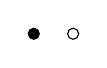
\begin{tikzpicture} \draw[fill=black] (0,0)circle(2pt); \draw[fill=white] (0.5,0)circle(2pt); \end{tikzpicture}\\
It is given by
\begin{align*}
	J&=\frac{\mmatrix{N-2 \\ M-1}}{\mmatrix{N\\ M}}\\
	&=\frac{\# \text{ configurations for $M-1$ particles on the remaining $N-2$ sites}}{\# \text{ configurations}}\\
	&=\frac{M}{N}\frac{N-M}{N-1}
\end{align*}
In the limit $N,M\to\infty,\ \frac{M}{N}=\rho$ we get $J=\rho(1-\rho)$\\
This result agrees to the most naive approach, a simple product ansatz, since:
\begin{equation*}
	J=\left\langle n_i(1-n_{i+1})\right\rangle = \langle n_i\rangle -\langle n_in_{i+1}\rangle\underset{\text{PA}}{\approx} \overset{\rho}{\langle n_i\rangle}-\overset{\rho}{\langle n_i\rangle}\overset{\rho}{\langle n_{i+1}\rangle}=\rho(1-\rho)
\end{equation*}
\textbf{\underline{\smash{Open systems}}}\vspace{3mm}\\
We now consider a system that is coupled to two particle reservoirs.
\begin{figure}[H]
	\centering
	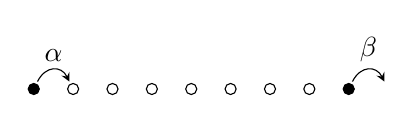
\begin{tikzpicture}
		\foreach \s [count=\x] in {black,white,white,white,white,white,white,white,black}{
			\draw[fill=\s] ({\x/2-0.5},0)circle(2pt)coordinate(a\x);
		}
		\draw[->,>=stealth,shorten <= 3pt, shorten >= 3pt] (a1) .. controls +(0.15,0.3) and +(-0.15,0.3) .. (a2)node[midway,above]{$\alpha$};
		\draw[->,>=stealth,shorten <= 3pt, shorten >= 3pt] (a9) .. controls +(0.15,0.3) and +(-0.15,0.3) .. ++(0.5,0)node[midway,above]{$\beta$};
	\end{tikzpicture}
\end{figure}
\noindent The particle dynamics is described by the ASEP rules in the bulk. They may enter the system at site 1 with rate $\alpha$ and leave it at site $N$ with rate $\beta$. We introduce the occupation number $n_i=\left\{0,1\right\}$ ($n_i=0 (1)$: site $i$ is empty (filled))\\
The particle number evolves as
\begin{equation*}
	\frac{dn_i(t)}{dt}=n_{i-1}(t)(1-n_i(t))-n_i(t)(1-n_{i+1}(t))
\end{equation*}
Averaging over different histories, we get: 
\begin{equation*}
	\frac{d\langle n_i(t)\rangle}{dt}=\left\langle n_{i-1}(1-n_i)\right\rangle -\left\langle n_i(1-n_{i+1})\right\rangle
\end{equation*}
\textbf{\underline{\smash{Remark}}}: Please note that this \textbf{exact} expression relates densities to two-point correlation functions $\left\langle n_in_{i+1}\right\rangle \ \& \ \left\langle n_{i-1}n_i\right\rangle$ This implies that a hierarchy of correlation functions has to be solved in order to calculate exact expressions of the density.\\
\begin{figure}[H]
	\centering
	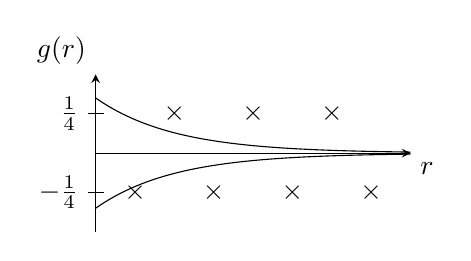
\begin{tikzpicture}[>=stealth]
		\draw[->] (0,-1)--(0,1)node[above left]{$g(r)$};
		\draw[->] (0,0)--(4,0)node[below right]{$r$};
		\draw (-0.1,0.5)node[left]{$\frac{1}{4}$}--(0.1,0.5)(-0.1,-0.5)node[left]{$-\frac{1}{4}$}--(0.1,-0.5);
		\foreach \x [count=\y] in {-1,1,-1,1,-1,1,-1}{
			\draw ({\y/2},{\x/2})node{$\times$};
		}
		\draw[domain=0:4,samples=50] plot(\x,{0.7*exp(-\x)})plot(\x,{-0.7*exp(-\x)});
	\end{tikzpicture}
	\begin{equation*}
		g(i,r)=\left\langle n_i n_{i+r}\right\rangle -\rho^2
	\end{equation*}
\end{figure}
\noindent The equation above holds for the time evolution of the density in the bulk. The complete set of equations is given by
\begin{equation*}
	\frac{d\langle n_i\rangle}{dt}=\begin{cases} \alpha\langle 1-n_1\rangle -\langle n_1(1-n_2)\rangle & i=1\\ \langle n_{i-1}(1-n_i)\rangle - \langle n_i(1-n_{i+1})\rangle & 1<i<N\\ \langle n_{N-1}(1-n_N)\rangle - \beta\langle n_N\rangle & i=N\end{cases}
\end{equation*}
The steady state of the open system is in general non-trivial. Most elegantly it can be obtained by a matrix method.\\
The key idea is to write the probability of a given configuration $\vec{n}$ as a product of matrices.
\begin{equation*}
	P_N(\vec{n})=\frac{1}{Z_N}\langle W | \prod\limits_{i=1}^N n_iD + (1-n_i)E|V\rangle
\end{equation*}
where $D,E$ are matrices and $\langle W | , | V\rangle$ auxiliary vectors, and $Z_N$ denotes the normalization constant.\vspace{2mm}\\
\textbf{\underline{\smash{Example}}}: \tikz \foreach \x [count=\y] in {white,white,black,white} \draw[fill=\x] ({\y/2},0)circle(2pt); $\leadsto$ $P(0010)=\frac{1}{Z_4}\langle W| EEDE|V\rangle$\\
The normalisation constant $Z_N$ makes sure that the sum of all weights is normalized, $\sum\limits_n P(\vec{n})=1$. It is given by
\begin{equation*}
	Z_N=\langle W| (D+E)^N|\rangle = \langle W | C^N | E\rangle \text{ where } C=D+E
\end{equation*}
By using the matrix representation we get:
\begin{equation*}
	\langle n_i\rangle = \frac{1}{Z_N}\langle W | C^{i-1}DC^{N-i}|V\rangle
\end{equation*}
as average value of the density at site $i$, since $\langle n_i\rangle$ is the relative weight of all configurations with an occupied site $i$. Similarly the current between site $i$ and $i+1$ is given by
\begin{equation*}
	\langle J_i\rangle = \frac{1}{Z_N}\langle W | C^{i-1}DEC^{N-i-1}|V\rangle
\end{equation*}
As a result of mass conservation in the bulk we have $\langle J_i\rangle =\langle J\rangle = const.$\\
This implies that:
\begin{equation*}
	\alpha \langle E C^{N-1}\rangle = \langle DEC^{N-2}\rangle \cdots
\end{equation*}
From the bulk we get $(DE)C=C(DE)$. It turns out that the simplest solution $DE=E+D$ which fulfills the commutation relation is correct. Therefore, we get $\langle J_i\rangle=J =\frac{Z_{N-1}}{Z_N}$\\
The set of equations is completed by the boundaries via $DE=D+E;\ \langle W | E = \alpha^{-1}\langle W |;\ D|V\rangle = \beta^{-1}|V\rangle$.
